\chapter{Resultados e Discussão}
\label{ch:Resultados}

Este capítulo é destinado à exposição dos resultados do sistema de classificação de tipografias, contendo a análise e discussão destes no caso da utilização dos dois diferentes modelos classificadores, SVM e Floresta Aleatória.

\section{Classificação das Tipografias}

O sistema desenvolvido deve receber uma imagem e indicar a qual tipografia o caractere presente na imagem pertence, dentre aquelas escolhidas para compor o projeto. Sendo assim, as possíveis classes para as imagens são:

\begin{enumerate}
\item Adobe Jenson
\item Adobe Garamond
\item Baskerville
\item Didot
\item Clarendon Bold
\item Franklin Gothic URW Demi
\item Helvetica
\item Futura Book
\item Gill Sans
\end{enumerate}

Como descrito no capítulo anterior, o resultado da classificação das tipografias foi mensurado a partir de testes de predição utilizando validação cruzada e computando o índice de acerto variadas vezes. Além disso, o sistema foi sendo desenvolvido com o banco de imagens sendo incrementado de tipografia a tipografia e, em cada passo, realizada a validação cruzada e os testes de predição, bem como calculado o índice de acerto de classificação desse estágio. Todos esses dados são explicitados nas seções a seguir.

\subsection{Utilizando Support Vector Machine}

Primeiramente, utilizou-se para extração de atributos o modelo LBP e, para o classificador, o modelo linear SVM. Na tabela \ref{tab:svmResults} pode-se verificar o resultado de índice de acerto de classificação obtido mediante a utilização de banco de imagens de diferentes versões. Além disso, o leitor pode acompanhar na Figura \ref{fig:graficoSVM} o histórico do índice de acerto do sistema classificador utilizando os modelos citados. Vale ressaltar que, em algoritmo implementado anteriormente, as tipografias presentes em cada etapa eram adicionadas arbitrariamente no banco de imagens, o que poderia gerar alterações nos resultados finais. Sendo assim, implementou-se uma adição aleatória de cada tipografia no banco de imagens, repetindo o processo dez vezes e calculando sua média e desvio padrão.

%%% Tabela

%\begin{table}[h]
% \centering
% \begin{tabular}{l|c|c|c|c|c|c|c|c|c|c}
%    Quantidade de tipografias  & 2 & 3 & 4 & 5 & 6 & 7 & 8 & 9\\ no banco de imagens & & & & & & & & \\
%	\hline
%	Helvetica & X & X & X & X & X & X & X & X   \\
%	Garamond & X & X & X & X & X & X & X & X  \\
%	Clarendon &  & X & X & X & X & X & X & X    \\
%	Futura &  &  & X & X & X & X & X & X  \\
%	Baskerville &  &  &  & X & X & X & X & X    \\
%	Didot &  &  &  &  & X & X & X & X    \\
%	Gill Sans &  &  &  &  &  & X & X & X   \\
%	Jenson &  &  &  &  &  &  & X & X  \\
%	Franklin Gothic &  &  &  &  &  &  &  & X  \\
%	\hline
%	Acurácia [\%] & 94,2 & 83,16 & 64,47 & 57,58 & 55,94 & 50,44 & 48,15 & 45,53 \\
%	Desvio padrão [\%] & 2 & 5 & 4 & 5 & 2 & 2 & 3 & 3\\
% \end{tabular}
% \caption{Resultados de acurácia em testes de validação cruzada do sistema classificador utilizando o modelo SVM, avaliado com banco de imagens em processo de incrementação tipografia à tipografia - \textbf{Fonte:} Autora}
% \label{tab:svmResults}
%\end{table}



\begin{table}[h]
 \centering
 \begin{tabular}{l|c|c|c|c|c|c|c|c|c|c}
    Quantidade de tipografias  & 2 & 3 & 4 & 5 & 6 & 7 & 8 & 9\\ no banco de imagens & & & & & & & & \\
	\hline
	Índice de acerto [\%] & 82,54 & 71,05 & 67,77 & 57,74 & 56,33 & 50,84 & 48,59 & 45,17 \\
	Desvio padrão [\%] & 23 & 23 & 14 & 9 & 9 & 4 & 5 & 0\\
 \end{tabular}
 \caption{Resultados de índice de acerto da classificação em testes de validação cruzada do sistema classificador utilizando o modelo SVM, avaliado com banco de imagens em processo de incrementação tipografia à tipografia.}
 \label{tab:svmResults}
\end{table}

%%% gráfico

\begin{figure}[H]
 \centering
  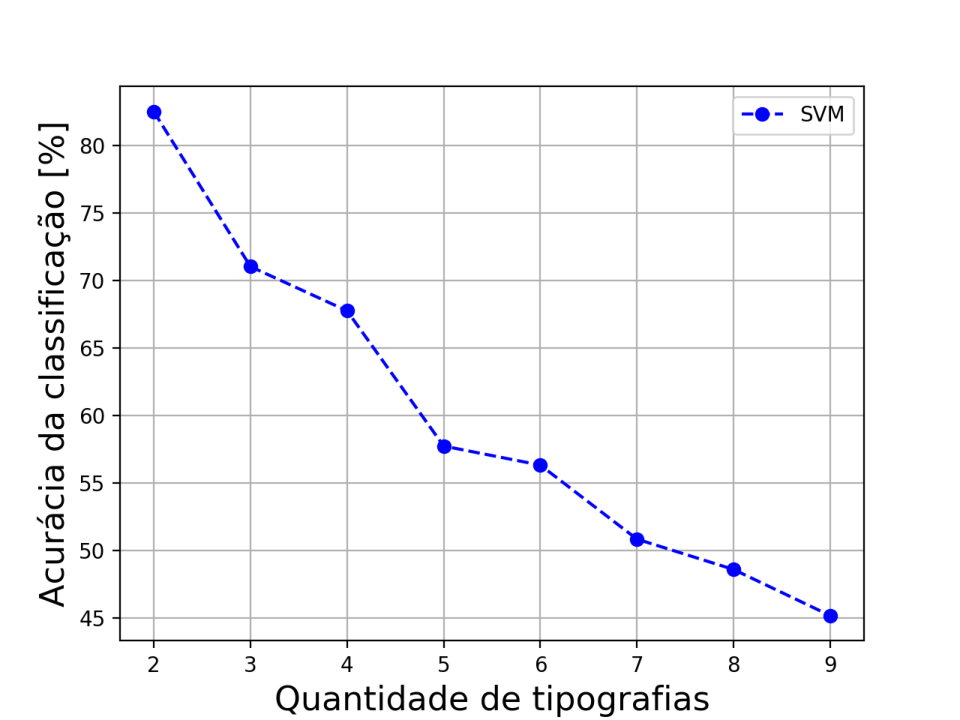
\includegraphics[width=0.7\linewidth]{figuras/graficosvm.pdf}
  \caption{Gráfico do desempenho do sistema classificador com o modelo SVM em relação à quantidade de tipografias presentes no banco de imagens.}
  \label{fig:graficoSVM}
\end{figure}

Percebe-se que, a cada incremento no banco de imagens, o nível de acerto da classificação é comprometido, chegando a 45,17\%, desvio padrão de 3\%, com banco de imagens com as nove tipografias. Diante do índice de acerto de classificação baixo para esta aplicação e, além disso, em comparação com trabalhos similares com índices de 85\% e 96,91\%, decidiu-se aplicar outro modelo classificador \citeC{la1999} \citeC{zramdini1998}. O resultado ruim pode ser fruto de uma sensibilidade do modelo SVM quanto aos atributos (dados) que lhe são fornecidos durante a etapa de treinamento \citeC{lorena2007}. Isto pode ser indicado, por exemplo, pelos valores altos encontrados no cálculo do desvio padrão durante os testes com o algoritmo SVM. Além disso, como já comentado anteriormente, a classificação é dificultada diante do alto grau de similaridade entre algumas tipografias presentes no projeto.

A SVM com \textit{kernel} linear foi aquela que obteve melhor resultado apesar de vários treinamentos da máquina terem sido efetuados com outras opções de \textit{kernel}, que podem ser vistos na Tabela \ref{tab:svmkernelResults}. Implementações com modelos não-lineares foram realizados somente no estágio final do banco de imagens, ou seja, com conjunto de nove tipografias.

\begin{table}[h]
 \centering
 \begin{tabular}{l|c|c}
    Kernel & Índice de Acerto [\%] & Desvio Padrão [\%]\\
	\hline
	Linear &  45,17 & 0 \\
	RBF & 37,28 & 4 \\
	Polinomial & 18,01 & 6  \\
	Sigmoidal & 35,61 & 5 \\
 \end{tabular}
 \caption{Índices de acerto da classificação em testes de validação cruzada do sistema com o modelo SVM avaliado com diferentes \textit{kernels} em banco de imagens com nove tipografias.}
 \label{tab:svmkernelResults}
\end{table}

Vale notar que a SVM linear obtém bom desempenho como classificador em conjuntos de dados com distribuição linear, ou que se aproximem desse padrão. Já no caso da utilização de \textit{kernel} não-linear, o conjunto de treinamento é mapeado para um espaço com dimensão superior e que seja mais suscetível à uma separação linear das classes \citeC{lorena2007}.

No entanto, os dois casos possuem um grau de dependência da distribuição do conjunto original de dados para que apresentem bom desempenho na classificação. Além disso, como pode-se perceber por sua característica linear intrínseca, o modelo SVM foi concebido como um classificador binário e, posteriormente, adaptado para conjuntos não-lineares em casos de multi-classificação \citeC{boser1992}. Dessa forma, a utilização da SVM nesse caso depende de uma série de parâmetros que devem ser bem ajustados para que ocorra a separação linear de forma ótima, o que dificulta sua utilização, fator que pode ter sido decisivo em seu desempenho neste projeto.

Portanto, para continuar empregando o classificador SVM, um modelo mais robusto de extração de atributos deveria ser utilizado, o que seria também uma opção para implementação do sistema. Porém, optou-se por manter o LBP para extração de atributos devido ao seu baixo custo computacional e rapidez de execução, critério importante no cenário de grande volume de dados e também por ser uma aplicação interativa, em se tratando de um produto final.



É ainda importante enfatizar a influência do conjunto de dados composto para o treinamento e testes no caso de aprendizado de máquina. Como descrito no capítulo anterior, o primeiro banco de imagens criado para treinamento e testes do sistema classificador comprometeu severamente o índice de acerto da classificação realizada pelo sistema. A Tabela \ref{tab:svmResults2} apresenta uma comparação entre os resultados obtidos com o banco de imagens precedente e o banco de imagens após maior refinamento. Vale ressaltar que o banco de imagens anterior foi desenvolvido apenas até conter quatro tipografias. Além disso, a SVM Linear foi o único modelo utilizado nessa avaliação.

\begin{table}[H]
 \centering
 \begin{tabular}{l|c|c|c|c|c|c|c|c|c|c}
    Quantidade de tipografias  no banco de imagens  & 2 & 3 & 4 \\
	\hline
	Helvetica & X & X & X  \\
	Garamond & X & X & X \\
	Clarendon &  & X & X \\
	Futura &  &  & X  \\
	\hline
	Índice de Acerto no Banco Antigo[\%] & 91,95 & 76,83 & 59,38 \\
	Desvio padrão [\%] & 2 & 2 & 2\\
	\hline
	Índice de Acerto no Banco Melhorado[\%] & 94,2 & 83,16 & 64,47 \\
	Desvio padrão [\%] & 2 & 5 & 4 \\
 \end{tabular}
 \caption{Resultados comparativos de índice de acerto da classificação em testes de validação cruzada do sistema classificador utilizando o modelo SVM linear, avaliado com banco de imagens antes e depois do refinamento, em processo de incrementação tipografia à tipografia, até quatro tipografias.}
 \label{tab:svmResults2}
\end{table}

\subsection{Utilizando Floresta Aleatória}

O segundo classificador utilizado foi o Floresta Aleatória, ainda com o modelo LBP para extração de atributos das imagens. Assim como na primeira versão do sistema, o modelo classificador foi treinado com oito versões do banco de imagens. A primeira versão é composta de duas tipografias que são suficientemente distintas entre si e então, a cada versão, o banco de imagens é incrementado com um conjunto de imagens de uma das tipografia presentes no projeto. Os resultados de índice de acerto da classificação performada pelo sistema utilizando Floresta Aleatória como classificador são expostos na Tabela \ref{tab:rfcResults}. Na Figura \ref{fig:grafico2}, pode-se ver a comparação dos resultados do classificador SVM e do classificador Floresta Aleatória a medida em que o banco de imagens foi sendo incrementado.


%%% Tabela

%\begin{table}[h]
% \centering
% \begin{tabular}{l|c|c|c|c|c|c|c|c|c|c}
%    Quantidade de tipografias  & 2 & 3 & 4 & 5 & 6 & 7 & 8 & 9\\ no banco de imagens & & & & & & & & \\
%	\hline
%	Helvetica & X & X & X & X & X & X & X & X   \\
%	Garamond & X & X & X & X & X & X & X & X  \\
%	Clarendon &  & X & X & X & X & X & X & X    \\
%	Futura &  &  & X & X & X & X & X & X  \\
%	Baskerville &  &  &  & X & X & X & X & X    \\
%	Didot &  &  &  &  & X & X & X & X    \\
%	Gill Sans &  &  &  &  &  & X & X & X   \\
%	Jenson &  &  &  &  &  &  & X & X  \\
%	Franklin Gothic &  &  &  &  &  &  &  & X  \\
%	\hline
%	Acurácia [\%] & 99,27 & 95,38 & 91,54 & 87,82 & 87,96 & 85,09 & 85,03 & 84,87 \\
%	Desvio padrão [\%] & 0 & 2 & 1 & 3 & 2 & 3 & 2 & 3\\
 %\end{tabular}
 %\caption{Resultados de acurácia em testes de validação cruzada do sistema com o modelo Floresta Aleatória, avaliado com banco de imagens em processo de incrementação tipografia à tipografia.}
 %\label{tab:rfcResults}
%\end{table}

\begin{table}[H]
 \centering
 \begin{tabular}{l|c|c|c|c|c|c|c|c|c|c}
    Quantidade de tipografias  & 2 & 3 & 4 & 5 & 6 & 7 & 8 & 9\\ no banco de imagens & & & & & & & & \\
	\hline
	Índice de acerto [\%] & 95,78 & 93,40 & 92,74 & 88,86 & 88,79 & 86,47 & 86,24 & 84,91 \\
	Desvio padrão [\%] & 9 & 7 & 3 & 3 & 5 & 2 & 2 & 0\\
 \end{tabular}
 \caption{Resultados de índice de acerto da classificação em testes de validação cruzada do sistema com o modelo Floresta Aleatória, avaliado com banco de imagens em processo de incrementação tipografia à tipografia.}
 \label{tab:rfcResults}
\end{table}

%%% gráfico


Sendo assim, o resultado final obtido para a classificação das nove tipografias apresentou um índice de acerto de 84,91\%, com desvio padrão de 3\%. O desempenho encontrado foi superior ao caso anterior, elevando o índice de acerto do sistema classificador. Apesar de ainda ser passível de melhoria, o desempenho foi similar ao encontrado em trabalho semelhante, que apresentou índice de acerto de 85\%, o que pode ser considerado adequado para um primeiro estágio no momento \citeC{la1999}.

\begin{figure}[H]
 \centering
  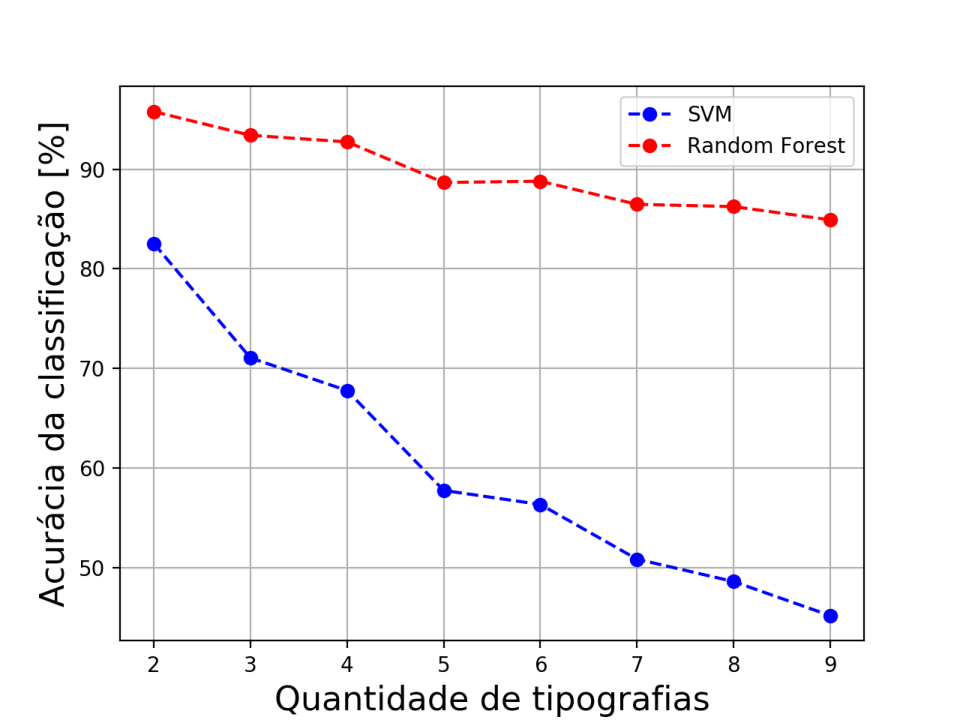
\includegraphics[width=0.7\linewidth]{figuras/graficosvmrfc.pdf}
  \caption{Gráfico do desempenho do sistema classificador com os dois modelos utilizados, SVM e Floresta Aleatória, em relação à quantidade de tipografias presentes no banco de imagens.}
  \label{fig:grafico2}
\end{figure}

Nota-se a grande discrepância entre o desempenho do sistema empregando o classificador Floresta Aleatória e a SVM. Esse resultado pode ser derivado de vários aspectos, entre eles, o perfil do conjunto de dados necessário para garantir um bom funcionamento da SVM como classificador.


Em relação ao modelo classificador Floresta Aleatória, os motivos pelos quais sua aplicação resultou em um melhor desempenho podem estar relacionados à robustez do modelo em relação a ruídos, bem como à distribuição e características gerais do conjunto de dados de entrada na máquina \citeC{breiman2001}. Além disso, por se tratar de um modelo construído por árvores de decisão (\textit{decision trees}), possui uma capacidade ampliada para lidar com espaços de variadas dimensões e também com um número alto de amostras de treinamento. Sendo assim, o modelo Floresta Aleatória pode ser considerado como um modelo que é intrinsicamente ajustado para multi-classificação, fato que facilita a sua utilização no caso aqui apresentado.

%As SVMs lineares são eficazes na classificação de conjuntos de dados linearmente se- paráveis ou que possuam uma distribuição aproximadamente linear, sendo que a versão de margens suaves tolera a presença de alguns ruídos e outliers. Porém, há muitos casos em que não é possível dividir satisfatoriamente os dados de treinamento por um hiperplano. Um exemplo é apresentado na Figura 8a, em que o uso de uma fronteira curva seria mais adequada na separação das classes. \citeC{lorena2007}

%As SVMs lidam com problemas não lineares mapeando o conjunto de treinamento de seu espaço original, referenciado como de entradas, para um novo espaço de maior dimensão, denominado espaço de características (feature space) [15]. Seja Φ : X → I um mapeamento, em que X é o espaço de entradas e I denota o espaço de características. A escolha apropriada de Φ faz com que o conjunto de treinamento mapeado em I possa ser separado por uma SVM linear. (BOA FIGURA NO ARTIGO)
